\chapter{Evaluation}
\label{cha:evaluation}

To prove the project's usability, it has not only to be tested against a ``real'' setup; additionally, it also has to be tested against different settings. Since it was designed to be as unopinionated as possible, there are still challenges to face concerning the overall support of different third-party tools, like template engines, etc.

Nevertheless, a base repository for future building using the REST API is set up without much hassle. As the project features a generic Metalsmith instance for building and rendering the different website projects, a local installation setup might as well be useful prior to handing over the repository to the REST API. This might support fixing bugs, which are probably much easier detected, if the source code is at hand.

\section{Minimal requirements}
\label{sec:minimalrequirements}

For even being able to build a repository successfully, it has to consist of a ``valid'' Metalsmith project. This means, that a few requirements have to be met, such as the following:

\begin{itemize}
  \item A folder structure, which consists of at least a source folder inside the project root,
  \item a configuration file, either in YAML or JSON format and named \emph{\_config.*},
  \item and finally being hosted on GitHub as public repository.
  \item Furthermore, it must not rely on any other build tools (e.g. \emph{Gulp}\footnote{\url{http://gulpjs.com} -- Website of Gulp.js}, \emph{Webpack}\footnote{\url{https://webpack.js.org} -- Website of Webpack.}, etc\ldots), only Metalsmith is supported at this time.
\end{itemize}

\subsection{Configuration file}
\label{sec:minimalrequirements-configuration}
The configuration file is probably the most critical part in the repository's contents, as it is the only source for the build pipeline to obtain the setup instructions from. Since the Metalsmith CLI is able to render a project based on a single JSON configuration file and the API setup doesn't really differ, the format of the configuration needed by the REST API is nearly identical. Therefore, the configuration for a local Metalsmith installation and the one used for the project's build pipeline are very well interchangeable (see Program \ref{list:pipeline-config}).

\begin{program}
  \caption{\textbf{\_config.yml} -- a sample configuration file, containing some global configuration data, as well as a few Metalsmith plugin definitions.}
  \label{list:pipeline-config}
\lstinputlisting[language=ruby]{chapters/06-evaluation/_support/_config.yml}
\end{program}

Since the REST API is able to parse both YAML and JSON notations, it is up to the developer to choose what fits his/her needs best. Since Metalsmith only understands JavaScript, any YAML configuration is parsed to JSON by the API, prior to forking the child process. This makes sense in a way, as the build setting information is getting included in the general options object, which is handed over from the REST API to the build pipeline, where parts of it get stored in the database together with the build log.

\subsection{Local testing}
Having a local Metalsmith install at stake may not only support the developer in finding and fixing bugs, it also helps to constantly pursue a clean build setup. The remote build pipeline neither is configured to inform about any installed modules, nor is it able to independently draw any conclusions of the provided configuration file. The only way to communicate with any responsible developer, is to send E-Mails containing status messages, or to respond build log information from the database upon request.

Although caching is not available when testing locally, it is often the only way to fix the build tree in a way, that Metalsmith is able to produce a successful outcome again. The reason behind that is the fact, that developers often try to fix a bug using subsequent small code changes -- this requires multiple rebuilds to check if the effort succeeded. However, it is also possible to patch the code base by adding one commit after another and analyze the messages of the build log entries.

\section{Comparison}
\label{sec:comparison}

When trying to compare the project's build pipeline to standalone static site generators like Jekyll or Metalsmith, it has to be stated, that neither one of those requires a git repository, nor any sort of authorization (besides during their installation process possibly). Furthermore, Jekyll also provides a command line argument for setting up a base project (see ch. \ref{sec:jekyll-technology} on p. \pageref{sec:jekyll-technology}), so that hardly any time is lost before a content author actually is being able to start writing.

As this project initially was designed to support porting Jekyll projects to Metalsmith, it already requires a basic structure for being able to work with. However, when starting from scratch, the probably best advice is to set up a local project, which makes use of the Metalsmith CLI and then start porting the configuration to fit the REST APIs standards.

\subsection{Jekyll}
A Jekyll project, as already explained in ch. \ref{sec:jekyll-technology}, is entirely written in Ruby and sets up on the Liquid templating engine. As a configuration file, it requires a YAML file called \emph{\_config.yml} in the project root and supports parsing data from YAML, JSON and CSV files to usable site variables out of the box \cite[76]{dhillon2016}. A functional Jekyll project also has to be equipped with Liquid templates in the \emph{\_layouts} folder, together with a few more directories holding different contents resulting in various recycleable parts during the build process. As of Jekyll 3.2, most of these parts have gotten outsourced in different Ruby gems, thus being hidden to the public and making it harder to port them to other generator applications like Metalsmith \cite{JekyllDirectoryStructure}.

\subsubsection{Jekyll source repository}
Parallel to the development of this project, the Jekyll docs sources\footnote{\url{https://github.com/jekyll/jekyll/tree/master/docs} -- Jekyll docs section in the Jekyll repository on GitHub.} were ported the best possible for setting a benchmark for the usability of the REST API. To make this happen, a few major changes needed to be made in order to get a positive build result:

\begin{itemize}
  \item The root folder was put in the source folder, but \emph{\_data}, \emph{\_layouts} and \emph{\_includes} were left out. Additionally, all asset-containing folders were moved into the \emph{\_public} directory.
  \item Necessary plugins were installed and configured for correctly setting the render flow:
  \begin{itemize}
    \item metalsmith-date-in-filename,
    \item metalsmith-sass,
    \item metalsmith-collections,
    \item metalsmith-permalinks,
    \item and a few more\ldots
  \end{itemize}
  \item Due to the limitations of \emph{TinyLiquid}\footnote{\url{https://github.com/leizongmin/tinyliquid} -- TinyLiquid repository on GitHub.}, especially file paths in include and extend statements had to be adjusted.
  \item Some functionality still does not work without further engineering, for example the YAML files in the \_data directory, or gem-dependent tasks like generating the sitemap or managing redirects.
\end{itemize}

To conclude; it is possible to successfully render a Jekyll project using Metalsmith, although there are a lot of adjustments necessary beforehand, not to speak of the deficits of the TinyLiquid package. Therefore, the expected behaviour of the outcome is likely to differ heavily from the reality. The test repository for this evaluation was obviously uploaded on GitHub\footnote{\url{https://github.com/vorchdorfmedia/jekyll-docs} -- Test repository for porting a Jekyll project to Metalsmith.} and may be tested locally using the Metalsmith CLI.

\subsection{Metalsmith}
Since Metalsmith was chosen for use as static site generator within the REST API (see ch. \ref{sec:primarythoughts-generator} on p. \pageref{sec:primarythoughts-generator}), it should be used as the foundation framework for any website project, which should be built using the REST API in the future. Due to the fact that Metalsmith is yet another npm module built for Node.js, it also offers to act as part of any available build tool, such as Gulp, Webpack or else -- however, this is not supported (see ch. \ref{sec:minimalrequirements} on p. \pageref{sec:minimalrequirements}).

The main reason behind this limitation is, that automatically detecting a different or additional build setup is error-prone and may easily slow down the render process. Furthermore, Metalsmith offers a feature-rich API and the possibility of writing plugins\footnote{\url{http://www.metalsmith.io/\#writing-a-plugin} -- ``Writing a plugin'' section in Metalsmith's documentation.} to fit the developer's needs, thus making nearly any additional build tool obsolete. All that is left to do, is to publish any written plugin publicly available to npm and append it to the repository's configuration file for future use in the build pipeline. As a result, other developers may also download and/or enhance the plugin to keep it up to date.

\section{REST API}
\label{sec:restapi}
The REST API was built and designed as remote-acting standalone web application, running on Node's servers-side JavaScript engine. Apart from specificly reserved firewall ports, the project is only dependent on a Node.js install, every other dependency may be installed using npm, regardless on the used operating system.

By extending any desired Node.js Dockerfile\footnote{\url{https://hub.docker.com/\_/node/} -- Official repository for Node.js on Docker Hub.}, it may be even run as autonomous Docker container and therefore multiplied for better load balancing based on the current HTTP load extent.


%% Screenshot of console log output after running artillery
\begin{figure}[h] % h-ere, t-op, b-ottom, p-age
    \centering
    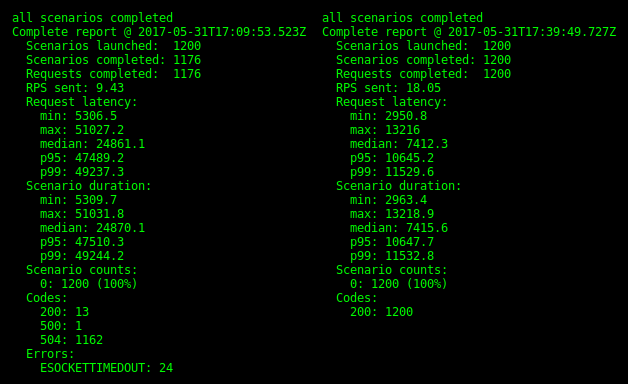
\includegraphics[width=0.9\textwidth]{pen_test.png}
    \caption{Screenshots of two command line outputs showing the results of the REST API being put under high HTTP load. During 60 seconds, the API had to face \emph{1200 requests} of 20 virtual clients created by Artillery. The test on the left was defined to include a single POST request triggering a new build cycle (with a full rebuild option) every time the API accepted a new connection. The results show the following: \emph{24} could not be handled at all, \emph{1162} resulted in gateway timeouts (GitHub blocks), but \emph{13} were handled successfully and returned with a \emph{200 OK} HTTP status code.}
    \label{fig:pen-test}
\end{figure}
%

%% Screenshot of the Mailgun result log
\begin{figure}[h] % h-ere, t-op, b-ottom, p-age
    \centering
    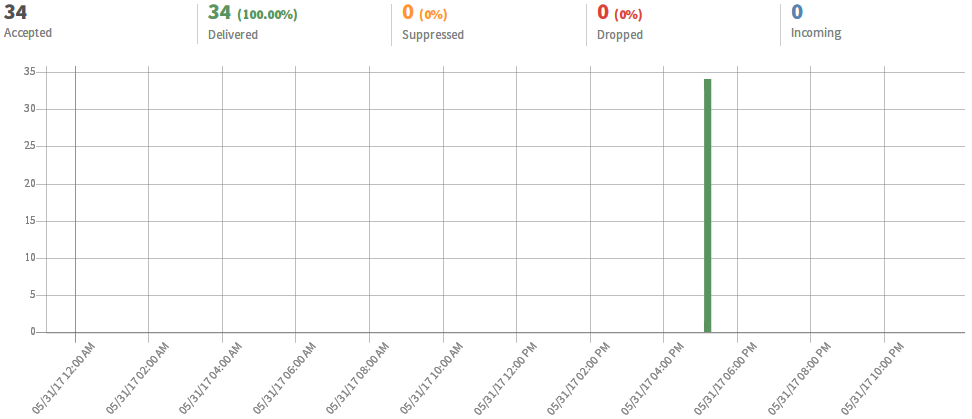
\includegraphics[width=0.9\textwidth]{mailgun_result.png}
    \caption{A screenshot showing the extent of the previous load-test (see fig. \ref{fig:pen-test}) in the Mailgun dashboard. Obviously, the build pipeline was triggered \emph{34} times, leading to the same number of E-Mails being sent. Out of this 34 E-Mails, \emph{8} showed a success message, whereas the others mostly failed due to other concurrent requests deleting the CWD as a preparation step prior to downloading the repository archive.}
    \label{fig:mailgun-result}
\end{figure}
%

\subsection{Load testing}
To evaluate the basic stability while handling multiple concurrent requests, the API was put under a high load test using Artillery\footnote{\url{https://artillery.io} -- Website of Artillery, a load testing toolkit.} (see fig. \ref{fig:pen-test}). Without any load balancing, nor any other high load supporting tool, 1200 POST requests triggered the build pipeline for a total duration of 60 seconds. As explained in the graphic's caption, the penetration test showed a success rate of roughly 1\%, a reasonable minimal response time of about 5 seconds but a terrible maximum response time of 51 seconds.

Of course, this data may not be interpreted as successful result in the first place, but it has to be stated, that the test was run on the endpoint causing the heaviest task in the system and most failure responses were effected by GitHub blocking most requests due to their rate abuse checking system.

The same test running on a much lighter task is showing a different picture; 1200 GET requests for receiving information about the latest build cycle had a response rate of 100\%. The response time ranged from 3 to 13 seconds, which is again a sign to not let a single application handle such an amount of requests without load balancing beforehand. In the end, it is safe to say, that the REST API may handle a reasonable amount of requests quite well on its own (e.g. requests triggered by GitHub webhooks), but consisting of multiple instances may be the best option for handling a significant amount of requests every once in a while.

\section{Caching}
\label{sec:caching}

In terms of caching, the build pipeline is best evaluated when assuming the best possible, as well as the worst possible case. As already explained in ch. \ref{sec:challenges-cachedetermination} on p. \pageref{sec:challenges-cachedetermination}, such scenarios would be on the one hand a commit only containing content changes (e.g. new or modified blog posts) and on the other hand a commit containing a modification of the default template. Since the default template is very likely to act as a dependency of nearly all content files, a full rebuild is inevitable.

\subsection{Initial build}
An initial build is necessary every time a repository was registered using the REST API, or the repository's previous build attempts constantly failed and no successful outcome was produced yet. Not only caring for the required folder structure, a successful build cycle also provides information for a subsequent rendering process by storing its head commit hash value in the build log on the database. Any following build attempt is able to forge upon the last successful build files.

Therefore it is a good advice to have a successful initial build ready as soon as possible, as future build cycles profit from an early render history and a best possible caching structure. By omitting an early registration to the REST API, any initial build cycle in the future will last a significant amount of time longer, due to continuous progression which is not able to make use of any cached file structure.

%% Graphic of MongoDB entries
\begin{figure} % h-ere, t-op, b-ottom, p-age
    \centering
    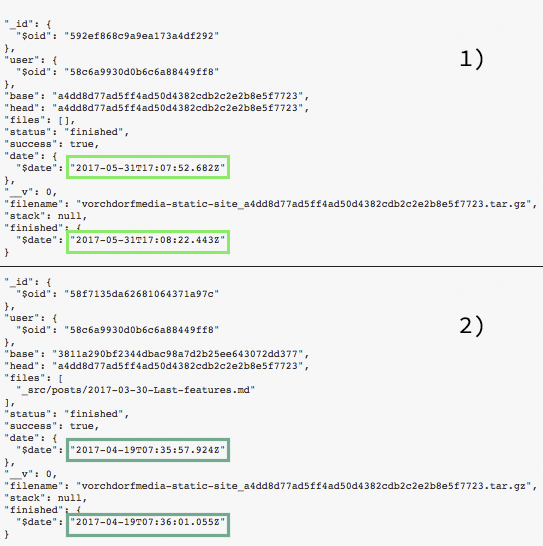
\includegraphics[width=0.9\textwidth]{caching_mongodb.png}
    \caption{Two screenshots of build log entries on the database showing the extent of ideal caching. Example \emph{1)} shows a forced rebuild during the load test (see fig. \ref{fig:pen-test}). Obviously there already happened some successful rendering cycles in the past, as \emph{base} and \emph{head} show the same commit hashes. The build lasted roughly 30 seconds and resulted in a successful archive file.\\
    Example \emph{2)} shows an earlier build, which made use of an available cache. The entry listed in the ``files'' array was the only file, which was rendered and added to the existing file structure. Therefore the build cycle lasted only 4 seconds.}
    \label{fig:caching-mongodb}
\end{figure}
%

\subsection{Caching strategy}
Since caching works most effectively if subsequent commits only contain content changes, the commit culture should be focused towards a content-only development, to make use of a long-lasting series of performant build cycles. Normally, this would be the standard for steady sites containing a significant amount of various information (e.g. FAQ-, support-, or documentation-sites), where constantly changing design decisions are not likely to play an important role. Concerning the need of a templating- or design change, the probably best advice is to collect commits containing such system files for as long as possible before actually merging them into the main branch and causing a longer lasting rebuild task, resulting in a major redesign.

Blogs are also likely to follow this kind of commit pattern, as usually a theme is set once, before subsequent blog posts are published. Using this type of scenario, the extent of ideal caching may be seen on fig. \ref{fig:caching-mongodb}. A rebuild, as well as an initial build at a later time is a lot more time consuming for resulting in a sane file structure, than a selectively rendered build result, which is able to get merged into an existing website root.

Thereby it is not important to check for any existing file structure, if any previously failed build attempt forced a rebuild due to its commit history, as the current build is always able to rely on the rendering result of the last successfully logged attempt.

\section{Outlook}
\label{sec:outlook}

Since this project has to be merely seen as a proof of concept, a few open points still remain. One of them would be the possibility of including it into a project workflow as a continuous integration service. By acting as an interface between GitHub and any deployment service, which is able to decompress a tar.gz archive, it would be the missing link for an automated update process to the web hosting service.

However, for extending the precision and usability of the REST API, some additional enhancements are necessary, where each of them is likely to form the extent of a project of its own.

\subsection{User experience}
\label{sec:outlook-userexperience}

To not only offer access to the REST API, but also a certain level of project management without relying on pure HTTP requests, it needs a graphical user interface. Furthermore, the current setup consists of a hard-coded access token for accessing certain data on GitHub -- this is not feasible for a multi-user system.

\subsubsection{Graphical user interface}
Through providing a graphical user interface (\emph{GUI}), a repository owner may not only have the possibility of a quick overview of his/her project, also managing a repository by adding/removing contributors authorized for triggering build cycles, as well as adjusting settings for any possible deployment strategy surely leverages the overall productivity. Moreover, build messages may be examined much easier and clearer.

Because of the REST API already being present, such a GUI may easily be built on top using different frontend libraries based on JavaScript. In the end, the API below will have to be extended for a few endpoints more. This not only enhances the overall functionality of the GUI, but also enables to provide the same functions to low level HTTP requests.

\subsubsection{GitHub authorization}
For making it possible to interact with repository data of any logged in user, he/she has to grant access somehow \cite{GithubAuthentication}. Normally this is done via a dialog in the browser, then the REST API receives an access token for making future requests without permanently asking the user for authorization, similar to the implemented OAuth 2.0 framework (see Sec. \ref{sec:foundation-express-oauth}).

\subsection{Cache improvement}
\label{sec:outlook-cacheimprovement}

Caching currently works by only comparing file paths, thus differentiating between system- and content files. Whereas this works fine for the vast majority of used repositories to a reasonable extent, the performance, as well as the reliability also depend on future improvements concerning the selective rendering algorithm.

\subsubsection{Frontmatter parsing}
The first approach for improving the overall caching performance would be an analysis of the frontmatter. As it is written in YAML and delimited using three dashes on the top and on the bottom \cite[77]{dhillon2016}, it should be very well parseable. Metalsmith already does that in order to provide different plugins with additional per-post metadata. However, since the list of cacheable files already has to be declared prior to creating the Metalsmith instance, making use of data parsed by Metalsmith would conflict the actual caching process.

This is aggravated by the fact that frontmatter does not always follow a fixed schema, so that every repository owner would have to introduce certain keys into a kind of tracking system on the REST API for supporting the caching algroithm with additional data.

\subsubsection{Machine learning}
\label{sec:chacheimprovement-machinelearning}
A much more performant approach would be the constant tracking of processed files and thereby creating a virtual network of dependencies within a respository. Based on the individual data of every website project, the conjunctions to various dependent files of a system file (e.g., a template) could be revealed. A precise detection of cacheable files could be refined more and more, resulting in the most performant build process possible.


